\chapter{Control and safety}
\label{ch:control}

\pkg{dharma_control} contains \code{control_mux_node}, the \textbf{only} publisher of the
robot's \topic{cmd_vel}. It arbitrates navigation (AUTO) and one operator source (REMOTE), keeps
every command inside the robot's envelope, limits it with a protective field on the 360° safety
scan and holds a latched e-stop with a hardware input and re-arm.

\begin{figure}[h]
  \centering
  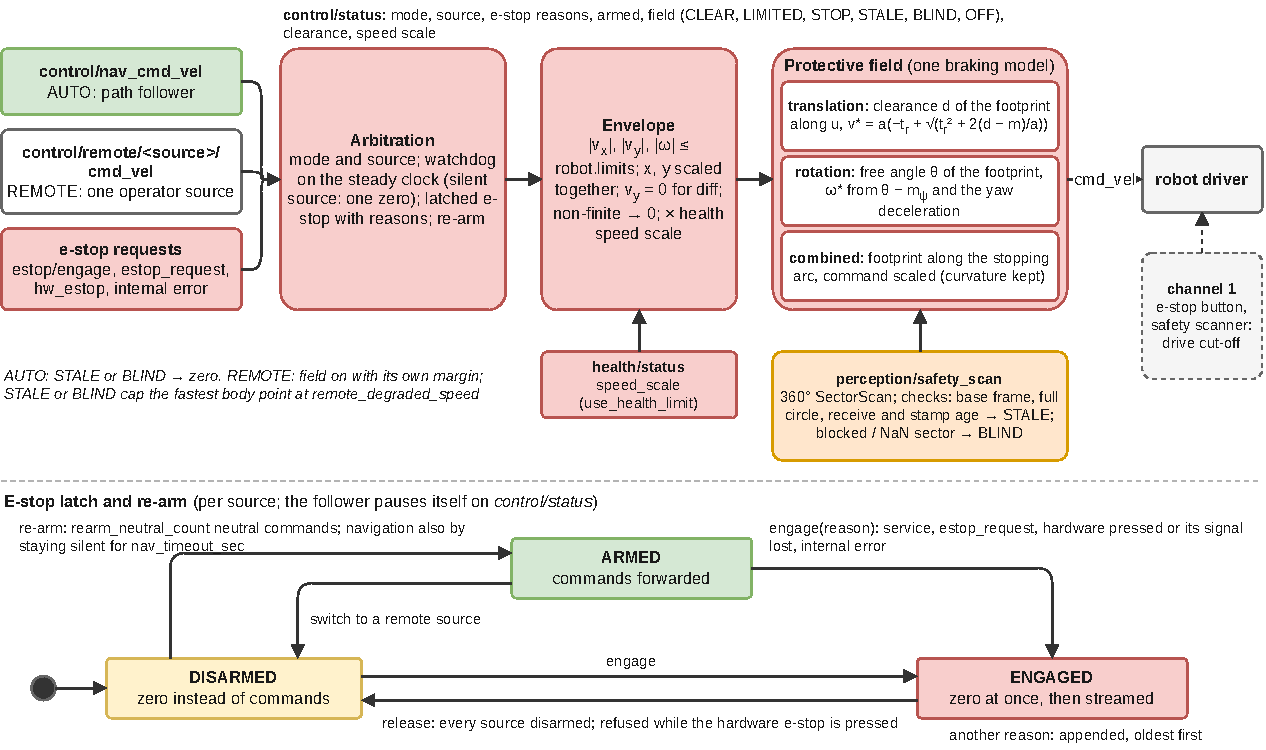
\includegraphics[width=\textwidth]{safety_pipeline}
  \caption{The safety layer and the e-stop latch with re-arm.}
  \label{fig:m-safety}
\end{figure}

\section{Two-channel safety architecture}
\label{sec:two-channel}

The control mux is a software safety function in Python over DDS. It is \emph{not} certified and
must never be the only protection of a robot that drives among people (finding C2). Products for
public spaces use two channels:

\begin{center}
\begin{tabularx}{\textwidth}{@{}p{0.18\textwidth}Xp{0.27\textwidth}@{}}
  \toprule
  Channel & What & Stops the robot by \\
  \midrule
  1 (hardware) & e-stop buttons and, where required, a safety-rated scanner or bumper wired to
    the drive's safe torque off or brake input, designed to ISO 13849-1~\cite{iso13849} (for
    example PL~d) or IEC 61508~\cite{iec61508}; ISO 13482~\cite{iso13482} applies to personal
    care robots & cutting the drive, independently of any software \\
  2 (\code{control_mux_node}) & envelope, protective field, watchdogs, latched software e-stop:
    smooth, early, configurable & publishing zero on \topic{cmd_vel} and streaming zero while
    engaged \\
  \bottomrule
\end{tabularx}
\end{center}

Wire channel~1's state to \topic{control/hw_estop} (Bool, true = pressed): while it is pressed
the software e-stop cannot be released, and after the button is released an operator still has
to release the software e-stop explicitly. With \param{hw_estop_timeout_sec} $> 0$ a silent
publisher of \topic{control/hw_estop} engages the e-stop (the signal is then required). The
driver must stop on its own command timeout, which covers a crash of the mux until it respawns.

\section{Pipeline}

\subsection{Arbitration}

AUTO forwards \topic{control/nav_cmd_vel}; REMOTE forwards
\topic{control/remote/<source>/cmd_vel} of the selected source only (\param{remote_sources},
default \texttt{[handheld, dashboard]}; review \#8: several operators on one topic).
\topic{control/set_mode} with the current mode and source is a no-op (review \#13); a change
publishes one zero and resets the watchdog; unknown modes or sources are rejected. The
\textbf{watchdog} gives the active source one zero when it is silent longer than
\param{nav_timeout_sec} or \param{remote_timeout_sec}. All timeouts and the e-stop hold run on the
steady clock: clock jumps and \code{use_sim_time} never disable them (review \#4).

\subsection{E-stop latch and re-arm}

\begin{itemize}
  \item \textbf{Engage.} \topic{control/estop/engage} (Trigger), \topic{control/estop_request}
    (String reason), \topic{control/hw_estop}, a silent hardware signal, or an internal error.
    Reasons accumulate, oldest first, without duplicates (review \#14). Zero is published at once
    and streamed at \param{estop_hold_hz}. Mode switches are allowed while engaged but forward
    nothing.
  \item \textbf{Release.} \topic{control/estop/release} (Trigger) is refused while the hardware
    e-stop is pressed; it clears the reasons and disarms every source. There is no
    \code{SetBool}: in 0.1 a default request released the e-stop and anyone could release
    anyone's e-stop (review \#3).
  \item \textbf{Re-arm.} At start, after a release and after switching to a remote source, a
    source is disarmed: it must send \param{rearm_neutral_count} consecutive neutral commands
    (every axis below \param{neutral_eps}) before anything it sends is forwarded, so a stick held
    during a release never moves the robot (review B3). Navigation also re-arms by staying silent
    for \param{nav_timeout_sec}.
  \item \textbf{Navigation pauses itself.} The mux never calls navigation services (review B3:
    the e-stop was resumed through \code{set_mode}); the follower reads \topic{control/status}:
    \code{estop} is a sticky pause reason there (cleared by \topic{navigation/resume}),
    \code{remote} a transient one.
\end{itemize}

\subsection{Envelope}

$|v_x| \le$ \param{max_vx}, $|v_y| \le$ \param{max_vy} (0 for \code{diff}), $|\omega| \le$
\param{max_wz} from \param{robot.limits}; $v_x$ and $v_y$ are scaled together, keeping the
direction. Any non-finite axis makes the command zero (review \#5: NaN limits disabled the
envelope). With \param{use_health_limit}, every axis is multiplied by \code{HealthStatus.speed_scale}
(stale health: no change). Commands are clamped before the field.

\subsection{Protective field}

AUTO always; REMOTE when \param{field.in_remote} (default true since 0.2.0, with
\param{field.remote_margin}). The model is speed and separation
monitoring~\cite{isots15066,marvel2016ssm} with the braking model of
Section~\ref{sec:braking}.

\textbf{Translation.} For the commanded direction $\hat{\vect{u}}$, the clearance $d_t$ is the
distance the footprint can move before touching a scan point
(\code{translation_clearance}): points ahead of the leading edge count when they lie within the
body corridor widened by \param{field.lateral_margin}; a point beside the body (behind the
leading edge, inside the corridor) or inside the footprint gives 0. The speed is limited to
$v^*(d_t - m)$ with $m$ = \param{field.margin}; below \param{field.min_speed} it stops. With
$a = 0.6$~m/s$^2$, $\tr = 0.25$~s and $m = 0.15$~m:
\begin{center}
\begin{tabular}{@{}lrrrr@{}}
  \toprule
  free distance $d_t$ & 0.3~m & 0.5~m & 1.0~m & 2.0~m \\
  allowed speed $v^*$ & 0.30~m/s & 0.52~m/s & 0.87~m/s & 1.35~m/s \\
  \bottomrule
\end{tabular}
\end{center}

\textbf{Rotation} (finding C1). In 0.1 only $v_x, v_y$ were scaled: a pure rotation passed
unchecked, although the corners of the footprint sweep the ring $r_{\mathrm{in}} < r \le
r_{\mathrm{c}}$ (0.28 to 0.49~m) and hit obstacles beside the robot. Now the free angle
$\theta_f$ (\code{rotation_room}: the ring points are rotated in 1° steps against the turning
direction until one enters the footprint; a point already inside gives 0) bounds the yaw rate:
$|\omega| \le \omega^*(\theta_f - m_\psi)$ with the yaw deceleration \param{max_yaw_accel} and
$m_\psi$ = \param{field.yaw_margin}; below \param{field.min_yaw_rate} it stops.

\textbf{Combined motion.} For $(v_x, v_y, \omega)$ the robot keeps the twist for $\tr$ and then
brakes both axes in proportion (the arc is kept) over $T_b = \max(v/a, |\omega|/\alpha)$. It covers
the constant-twist arc
\begin{equation}
  x(u) = \frac{v_x\sin\omega u - v_y(1 - \cos\omega u)}{\omega}, \quad
  y(u) = \frac{v_x(1 - \cos\omega u) + v_y\sin\omega u}{\omega}, \quad \psi(u) = \omega u
\end{equation}
up to $u = \tr + T_b/2$, exactly $D(v)$ on a straight line, plus an extension of
$\min(m/v, m_\psi/|\omega|)$. The footprint (widened by the lateral margin) is checked at poses
along the arc; a point already beside the body may be passed but not approached closer than
2~cm. If the first contact is at $u_c$, scaling by $s$ keeps the curvature and covers
$s\,\tr + s^2 T_b/2$, so the largest clear scale is
\begin{equation}
  s = \frac{-\tr + \sqrt{\tr^2 + 2\,T_b\,(u_c - u_{\mathrm{ext}})}}{T_b}.
\end{equation}

\subsection{Scan validation and degraded sensing}

\topic{perception/safety_scan} is accepted only in \param{robot.frames.base} with full-circle
coverage (review \#7). It is \code{STALE} when invalid, not received for
\param{field.scan_timeout_sec} (monotonic receive age) or when its stamp is older than
\param{field.scan_max_age_sec} or more than \param{field.scan_clock_tolerance_sec} in the future.
Any blocked or NaN sector makes it \code{BLIND} (review B1: an all-zero scan was read as clear).
\begin{itemize}
  \item AUTO: \code{STALE} or \code{BLIND} $\to$ zero; no scan at all $\to$ zero.
  \item REMOTE: the fastest point of the body ($v + |\omega| r_{\mathrm{c}}$) is capped at
    \param{field.remote_degraded_speed}; with a partly blind scan the field still applies to the
    points it sees, and a translation toward a blocked sector is refused.
\end{itemize}
\code{control/status} reports the field state (\code{CLEAR}, \code{LIMITED}, \code{STOP},
\code{STALE}, \code{BLIND}, \code{OFF}), the clearance and the applied speed scale.

\subsection{Fail-safe behaviour}

An exception in any callback engages the e-stop with the reason \texttt{internal error} and
publishes zero (review \#6); on shutdown the node publishes zero three times. Safety parameters
are read-only at runtime and validated at start (decelerations $> 0$, timeouts $> 0$, margins
$\ge 0$, finite values): the node refuses to start on a bad value (review \#5:
\texttt{max\_decel: 0} raised \code{ZeroDivisionError}).

\section{Safety case}
\label{sec:safety-case}

Hazards of the navigation function, their mitigations in the stack and the tests that verify
them. Test names are \code{file::function} in the package's \code{test/} directory (u: unit, r:
node test). The software mitigations are channel~2; residual risks need channel~1 or a sensor
the stack does not have.

\begin{small}
\begin{longtable}{@{}>{\raggedright}p{0.04\textwidth}>{\raggedright}p{0.25\textwidth}>{\raggedright}p{0.31\textwidth}>{\raggedright\arraybackslash}p{0.32\textwidth}@{}}
  \toprule
  & Hazard & Mitigation & Verification \\
  \midrule
  \endhead
  \bottomrule
  \endfoot
  H1 & collision with an obstacle ahead while driving & protective field translation limit
    with one braking model; follower motion guard; speed profile & u/\code{test_field::test_wall_ahead_limits_with_the_shared_stopping_model},
    u/\code{test_follower_safety::test_guard_checks_every_direction_of_the_footprint},
    sim E1 \todo{results} \\
  H2 & body corner hits an obstacle while turning in place & rotation limit from the swept ring
    (C1) & u/\code{test_field::test_rotation_next_to_an_obstacle_is_limited},
    r/\code{test_control_mux_node::test_field_limits_rotation_beside_an_obstacle} \\
  H3 & collision along a curved motion & stopping-arc check of combined motion &
    u/\code{test_field::test_combined_motion_checks_the_arc} \\
  H4 & blind LiDAR read as free space & BLOCKED sectors at the source, BLIND $\to$ zero in AUTO,
    creep in REMOTE (B1, F1) & u/\code{test_pipeline::test_blind_lidar_blocks_every_sector},
    u/\code{test_scan::test_all_sectors_zero_is_blind_not_clear},
    u/\code{test_field::test_blind_scan_stops_auto}, sim E2 \todo{results} \\
  H5 & perception stops publishing or lags & receive and stamp age checks, STALE $\to$ zero; BLOCKED
    watchdog in perception; respawn & u/\code{test_scan::test_receive_age_on_monotonic_time},
    u/\code{test_scan::test_header_age_old_and_future},
    r/\code{test_lidar_sector_node::test_silent_input_publishes_blocked_scans} \\
  H6 & scan in a wrong frame or with partial coverage & frame and coverage validation (\#7) &
    u/\code{test_scan::test_wrong_frame_is_rejected},
    u/\code{test_scan::test_partial_coverage_is_rejected} \\
  H7 & navigation keeps the last moving command (stop, crash, silence) & watchdog zero; zero on
    INACTIVE, stop and shutdown (F2, \#6) & u/\code{test_arbiter::test_watchdog_zeroes_once_per_silence},
    u/\code{test_follower::test_stop_zeroes_once_and_start_resumes},
    r/\code{test_control_mux_node::test_shutdown_hook_publishes_zeros} \\
  H8 & robot moves when an e-stop is released (held stick, resumed navigation) & re-arm with
    neutral commands; sticky \code{estop} pause in the follower (B3) &
    u/\code{test_arbiter::test_release_requires_rearm_and_never_forwards_the_held_command},
    u/\code{test_follower_safety::test_estop_is_sticky_and_remote_is_transient} \\
  H9 & e-stop released by a default or foreign request & Trigger services only; release refused
    while the hardware e-stop is pressed (\#3, C2) &
    u/\code{test_arbiter::test_hardware_estop_engages_and_blocks_release},
    r/\code{test_control_mux_node::test_hardware_estop_blocks_release} \\
  H10 & watchdog disabled by a clock jump or simulated time & steady-clock timers (\#4) &
    r/\code{test_control_mux_node::test_watchdog_and_hold_run_on_steady_time_with_sim_time} \\
  H11 & invalid safety parameter (zero deceleration, NaN limit) & validated typed configuration,
    read-only at runtime, refuse to start (\#5, F11) &
    r/\code{test_control_mux_node::test_bad_values_refuse_to_start},
    r/\code{test_control_mux_node::test_safety_parameters_are_read_only} \\
  H12 & software fault in the mux & e-stop on callback errors; respawn; driver command timeout
    (channel~1) & r/\code{test_control_mux_node::test_callback_error_engages_the_estop} \\
  H13 & floor seen as an obstacle or low obstacle hidden by body pitch & levelled height band,
    gravity-aligned \frm{odom} (P1, O1) &
    u/\code{test_filtering::test_pitched_body_does_not_see_the_floor},
    r/\code{test_lidar_sector_node::test_pitched_body_does_not_block_on_the_floor} \\
  H14 & low object near the robot below the lowest beam & obstacle memory in \frm{odom} (B4);
    residual: objects appearing inside the zone $\to$ pitched mount or near-field sensor &
    u/\code{test_memory_blindness::test_memory_keeps_an_object_the_sensor_no_longer_sees};
    residual risk documented \\
  H15 & negative obstacles (stairs down, edges) & not detected by the stack; residual: channel~1
    sensor or site restriction & -- \\
  H16 & planned path too narrow for the body when turning & radii from the footprint, oriented
    footprint check (N1) & u/\code{test_planning::test_door_narrower_than_the_body_is_refused},
    u/\code{test_planning::test_oriented_footprint_against_a_wall} \\
  H17 & robot pose stale or wrong (TF latency, clock offset) & TF age checks with prediction and
    stop, TF\_CLOCK; per-edge diagnosis in health & u/\code{test_follower_safety::test_tf_status_messages},
    u/\code{test_follower_safety::test_slightly_old_pose_is_predicted_with_the_twist} \\
  H18 & wrong localization correction moves the robot off its path & chi-square gate on the robot
    pose; OFF\_PATH stop (L1, \#1) &
    u/\code{test_estimator::test_gate_rejects_outliers_and_accepts_consistent_fixes_far_from_origin},
    sim E3 \todo{results} \\
  H19 & passing an obstacle at a stop point or while shifted & path shift limited by the measured
    offset; wait at stop points (F4, F6) & u/\code{test_shift::test_measured_offset_limits_the_speed},
    u/\code{test_follower::test_stop_point_with_an_obstacle_waits_instead_of_passing} \\
  H20 & software safety mistaken for a certified function & two-channel architecture documented;
    product safety case required (C2) & review of the product design \\
\end{longtable}
\end{small}

\section{Interfaces}

\begin{center}
\begin{tabularx}{\textwidth}{@{}p{0.36\textwidth}p{0.20\textwidth}X@{}}
  \toprule
  Interface & Type & \\
  \midrule
  \topic{cmd_vel} & Twist & out: the robot's command \\
  \topic{control/status} & ControlStatus, latched & on change and at \param{status_hz} \\
  \topic{control/nav_cmd_vel} & Twist & in: navigation (AUTO) \\
  \topic{control/remote/<source>/cmd_vel} & Twist & in: one per \param{remote_sources} entry \\
  \topic{perception/safety_scan} & SectorScan & in: 360° scan in the base frame \\
  \topic{control/estop_request} & String & in: engage with a reason \\
  \topic{control/hw_estop} & Bool & in: hardware e-stop, true = pressed \\
  \topic{health/status} & HealthStatus & in, with \param{use_health_limit} \\
  \topic{control/set_mode} & SetMode & \code{auto}, or \code{remote} with a source \\
  \topic{control/estop/engage}, \topic{control/estop/release} & Trigger & \\
  \bottomrule
\end{tabularx}
\end{center}

\section{Parameters}

All parameters of the mux are read-only at runtime. Measure \param{robot.limits.max_decel},
\param{max_yaw_accel} and \param{reaction_time} on the robot before it drives on its own.

% Generated by docs/manual/tools/reference.py; do not edit.
\begin{small}
\begin{longtable}{@{}>{\raggedright}p{0.25\textwidth}>{\raggedright}p{0.17\textwidth}>{\raggedright}p{0.10\textwidth}>{\raggedright}p{0.11\textwidth}>{\raggedright\arraybackslash}p{0.25\textwidth}@{}}
\toprule
Parameter & Default & Unit & Range & Description \\
\midrule
\endhead
\bottomrule
\endfoot
\multicolumn{5}{@{}l}{\textbf{control\_\allowbreak{}mux\_\allowbreak{}node}} \\
\code{mode}$^\dagger$ & \code{auto} &  & auto, remote & mode at start \\
\code{remote_sources}$^\dagger$ & [\code{handheld}, \code{dashboard}] &  &  & operator sources, each on control/remote/<source>/cmd\_\allowbreak{}vel; the first is the default \\
\code{nav_timeout_sec}$^\dagger$ & 0.5 & s & 0.02..5 & zero once when navigation is silent \\
\code{remote_timeout_sec}$^\dagger$ & 0.3 & s & 0.02..5 & zero once when the operator is silent \\
\code{estop_hold_hz}$^\dagger$ & 10 & Hz & 1..100 & zero commands while engaged \\
\code{rearm_neutral_count}$^\dagger$ & 3 &  & 1..100 & consecutive neutral commands the source must send before it drives again \\
\code{neutral_eps}$^\dagger$ & 0.01 & m/\allowbreak{}s, rad/\allowbreak{}s & 0.0001..0.2 & neutral: every axis below \\
\code{hw_estop_timeout_sec}$^\dagger$ & 0 & s & 0..10 & engage when control/hw\_\allowbreak{}estop is silent this long (0: the input is optional) \\
\code{use_health_limit}$^\dagger$ & false &  &  & scale every command by health/status speed\_\allowbreak{}scale \\
\code{health_timeout_sec}$^\dagger$ & 3 & s & 0.1..60 & older health/status is ignored \\
\code{status_hz}$^\dagger$ & 2 & Hz & 0.2..50 & control/status period (also on change) \\
\multicolumn{5}{@{}l}{\textbf{control\_\allowbreak{}mux\_\allowbreak{}node}} \\
\code{field.in_remote}$^\dagger$ & true &  &  & apply the field in REMOTE too (remote\_\allowbreak{}margin) \\
\code{field.margin}$^\dagger$ & 0.15 & m & 0..2 & gap kept to an obstacle in AUTO \\
\code{field.remote_margin}$^\dagger$ & 0.1 & m & 0..2 & gap kept to an obstacle in REMOTE \\
\code{field.lateral_margin}$^\dagger$ & 0.1 & m & 0..1 & extra width of the swept path \\
\code{field.human_speed}$^\dagger$ & 0.5 & m/\allowbreak{}s & 0..3 & assumed speed of a person walking toward the robot (ISO/TS 15066 separation) \\
\code{field.yaw_margin}$^\dagger$ & 0.1 & rad & 0..1 & turn kept short of a contact \\
\code{field.min_speed}$^\dagger$ & 0.02 & m/\allowbreak{}s & 0..0.5 & a slower allowed speed stops instead \\
\code{field.min_yaw_rate}$^\dagger$ & 0.05 & rad/\allowbreak{}s & 0..1 & a slower allowed turn stops instead \\
\code{field.remote_degraded_speed}$^\dagger$ & 0.15 & m/\allowbreak{}s & 0..1 & REMOTE with a stale or blind scan: fastest point of the body \\
\code{field.scan_timeout_sec}$^\dagger$ & 0.5 & s & 0.05..5 & scan receive age (monotonic) limit \\
\code{field.scan_max_age_sec}$^\dagger$ & 0.5 & s & 0.05..5 & scan header stamp age limit \\
\code{field.scan_clock_tolerance_sec}$^\dagger$ & 0.1 & s & 0..1 & accepted negative stamp age (clocks) \\
\end{longtable}
\end{small}

